\section{Production audit}
\label{sec:audit}

We measured 33 released tokenizers on parallel FLORES-200 devtest text. Nine have identical token counts to another tokenizer on all 36 FLORES languages we measured (for example, Phi-4, OLMo-2 and Granite-4.1 all match \texttt{cl100k}; Qwen3 matches Qwen2.5; SmolLM3 matches Llama-3). We treat them as aliases, leaving 24 distinct tokenizers (Figure~\ref{fig:audit}; full table in Appendix~\ref{app:audit}). Two further tokenizers are not in the audit: Kimi-K3 requires executing remote code to load, which we did not run, and Mistral-Large-3 loaded through HuggingFace as a degenerate tokenizer, so we excluded it. We classify each tokenizer by its own pre-tokenizer configuration, not by family. Four SentencePiece and WordPiece tokenizers (XLM-R, mT5, NLLB-200, IndicBERTv2) do not reproduce their input on decoding, so their low premiums are not comparable compression results; Figure~\ref{fig:audit} marks them, and we exclude them from the analysis below.

\paragraph{The pre-token floor.} Let $P$ be a tokenizer's pre-tokenizer and $T$ the tokenizer. Summed over the 1{,}012 devtest sentences, we call $|P(\text{ne})|/|T(\text{en})|$ the \emph{pre-token floor} of $T$. The Nepali/English premium cannot go below it under any vocabulary extension that keeps the pre-tokenizer and leaves English tokenization unchanged (\S\ref{sec:ceiling}). It is a lower bound, not a value that extension is guaranteed to reach.

\begin{figure}[t]
\centering
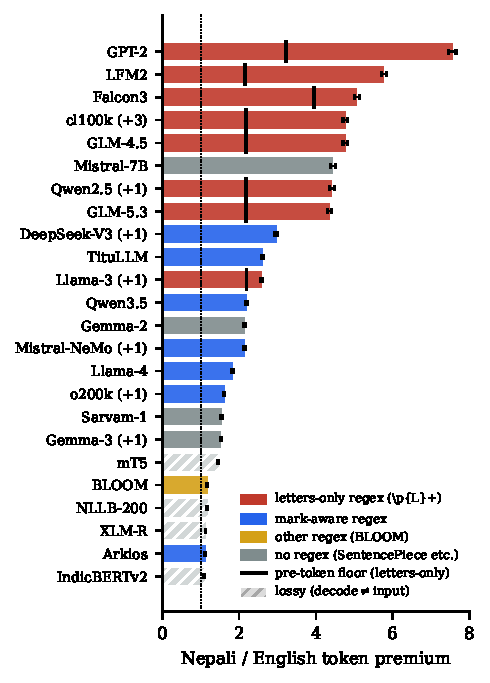
\includegraphics[width=\columnwidth]{fig_audit.pdf}
\caption{Nepali/English token premium of 24 distinct tokenizers (33 released tokenizers; ``+$n$'' counts aliases) on FLORES-200 devtest, with 95\% paired-bootstrap intervals. Black ticks mark the pre-token floor of each letters-only tokenizer: no vocabulary extension can move its bar to the left of the tick.}
\label{fig:audit}
\end{figure}

\paragraph{Every letters-only tokenizer has a floor of at least $2.15\times$.} Eight distinct tokenizers, covering 13 released names including GLM-5.3 and LFM2, use the letters-only class. Their premiums range from $2.58\times$ (Llama-3) to $7.55\times$ (GPT-2), and their pre-token floors from $2.15\times$ to $3.23\times$. Excluding GPT-2, a 2019 model that we include as a historical reference, the premiums of current letters-only models range from $2.58\times$ to $5.77\times$ (LFM2). The seven lossless tokenizers with a mark-aware regex range from $1.12\times$ (Arkios;~\citealp{regmi2026arkios}) to $2.97\times$ (DeepSeek-V3).

\paragraph{Decomposition.} Write the premium as
\begin{equation*}
\frac{|T(\text{ne})|}{|T(\text{en})|} = \underbrace{\frac{|P_{\text{rep}}(\text{ne})|}{|T(\text{en})|}}_{\text{base}} \cdot \underbrace{\frac{|P(\text{ne})|}{|P_{\text{rep}}(\text{ne})|}}_{\text{regex factor}} \cdot \underbrace{\frac{|T(\text{ne})|}{|P(\text{ne})|}}_{\text{vocabulary factor}},
\end{equation*}
where $P$ is the tokenizer's own pre-tokenizer and $P_{\text{rep}}$ is the repaired Llama-3 pattern (\S\ref{sec:method}), applied to every tokenizer. The numerator of the base term is therefore the same for all tokenizers; only the English token count varies. The base lies between $0.77$ and $0.80$ for every tokenizer, because English token counts barely differ. The regex factor is $0.98$--$1.02$ for mark-aware tokenizers, $2.77$--$2.79$ for the Llama-3/Qwen/\texttt{cl100k} pattern, and $4.06$ for the GPT-2 and Falcon3 patterns, which put every run of marks in a pre-token of its own. The vocabulary factor, tokens per pre-token, is what vocabulary extension can lower, and only down to 1.

Table~\ref{tab:decomp} shows where each tokenizer's premium comes from. For Llama-3 the vocabulary factor is $1.18$, the lowest in the audit: its 128k vocabulary already nearly covers Nepali pre-tokens, and almost all of its remaining premium is the regex factor. For Qwen and \texttt{cl100k} both factors matter. Among mark-aware tokenizers, the vocabulary factor varies from $1.43$ (Arkios, trained for Nepali) to $3.79$ (DeepSeek-V3): fixing the regex is necessary but does not by itself make a tokenizer good at Nepali.

\begin{table}[t]
\centering
\small
\setlength{\tabcolsep}{4pt}
\begin{tabular}{lrrrr}
\toprule
Tokenizer & Premium & Base & Regex & Vocab. \\
\midrule
GPT-2 & 7.55 & 0.80 & 4.06 & 2.34 \\
LFM2 & 5.77 & 0.78 & 2.77 & 2.68 \\
\texttt{cl100k} (+3) & 4.76 & 0.79 & 2.77 & 2.17 \\
Qwen2.5/3 & 4.42 & 0.78 & 2.79 & 2.03 \\
GLM-5.3 & 4.35 & 0.79 & 2.77 & 1.98 \\
Llama-3 & 2.58 & 0.79 & 2.77 & \textbf{1.18} \\
\midrule
DeepSeek-V3/V4 & 2.97 & 0.80 & 0.98 & 3.79 \\
Qwen3.5 & 2.20 & 0.78 & 1.02 & 2.76 \\
Llama-4 & 1.83 & 0.80 & 1.00 & 2.30 \\
\texttt{o200k} (+1) & 1.61 & 0.80 & 1.00 & 2.01 \\
Arkios & 1.12 & 0.79 & 0.99 & 1.43 \\
\bottomrule
\end{tabular}
\caption{Premium = base $\times$ regex factor $\times$ vocabulary factor, on FLORES-200 devtest, for 11 of the 15 letters-only and mark-aware tokenizers in the audit (top: letters-only; bottom: mark-aware). Arkios is from \citet{regmi2026arkios}. Vocabulary extension can only lower the last column, and not below 1.}
\label{tab:decomp}
\end{table}

\paragraph{Within-family changes.} Two families changed the regex between releases, together with the vocabulary. From Qwen3 to Qwen3.5 the Nepali premium halves, from $4.42\times$ to $2.20\times$; Qwen3.5's word branch is our repaired class with only the leading-character class left unchanged. \citet{land2026smallbugs} reported this change for Hindi. From Llama-3 to Llama-4 (which adopts \texttt{o200k}'s pattern) the premium falls from $2.58\times$ to $1.83\times$. In both cases the vocabulary also grew, so these are corroborating observations, not controlled comparisons; \S\ref{sec:compression} provides the controlled one.

\paragraph{Broken syllables.} Many Nepali tokens begin with a combining mark, which no well-formed Devanagari syllable does: 55\% of Llama-3's Nepali tokens, 32\% of Qwen3's and 30\% of \texttt{cl100k}'s (Appendix~\ref{app:audit}). The rate does not track the regex class. Mark-aware tokenizers show similar rates (26\% for \texttt{o200k}, 55\% for TituLLM, which keeps Llama-3's merges), because BPE also splits within words. \S\ref{sec:compression} shows how the rate moves under each retrofit.
